\appendix
    
\chapter{Resultados del Benchmark en Entorno Local (Compu Juan)}
\label{appendix:local}
En este anexo se presentan las tablas de tiempos, speedup y eficiencia obtenidos en el entorno local. 

\begin{figure}[H]
    \centering
    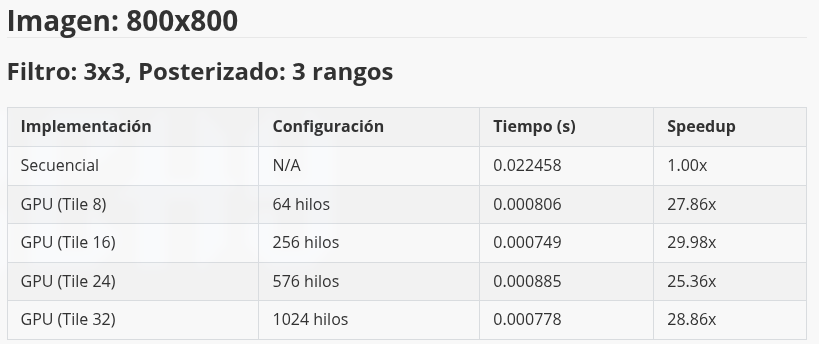
\includegraphics[width=1\textwidth]{resources/800gpu3x3.png}
    \caption{Resultados del benchmark en entorno local para imagen de 800x800, filtro 3x3 y 3 rangos de posterización.}
    \label{fig:800_local_3x3_3}
\end{figure}


\begin{figure}[H]
    \centering
    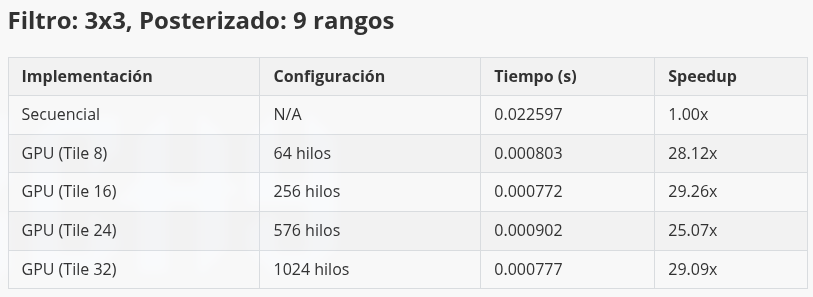
\includegraphics[width=1\textwidth]{resources/800gpu3x9.png}
    \caption{Resultados del benchmark en entorno local para imagen de 800x800, filtro 3x3 y 9 rangos de posterización.}
    \label{fig:800_local_3x3_9}
\end{figure}

\begin{figure}[H]
    \centering
    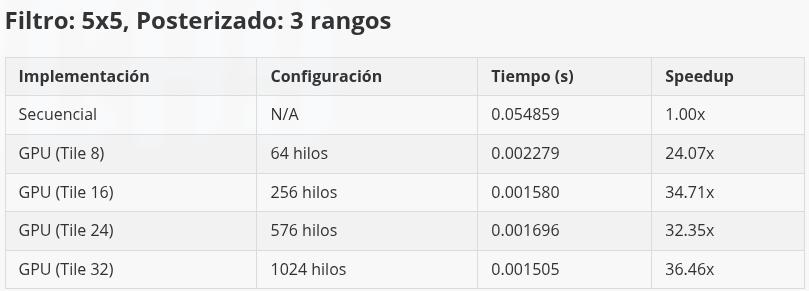
\includegraphics[width=1\textwidth]{resources/800gpu5x3.png}
    \caption{Resultados del benchmark en entorno local para imagen de 800x800, filtro 5x5 y 3 rangos de posterización.}
    \label{fig:800_local_5x5_3}
\end{figure}


\begin{figure}[H]
    \centering
    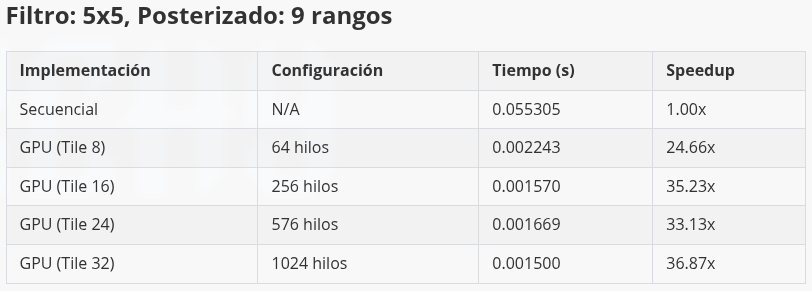
\includegraphics[width=1\textwidth]{resources/800gpu5x9.png}
    \caption{Resultados del benchmark en entorno local para imagen de 800x800, filtro 5x5 y 9 rangos de posterización.}
    \label{fig:800_local_5x5_9}
\end{figure}

% -------------------------------------------------------------------

\begin{figure}[H]
    \centering
    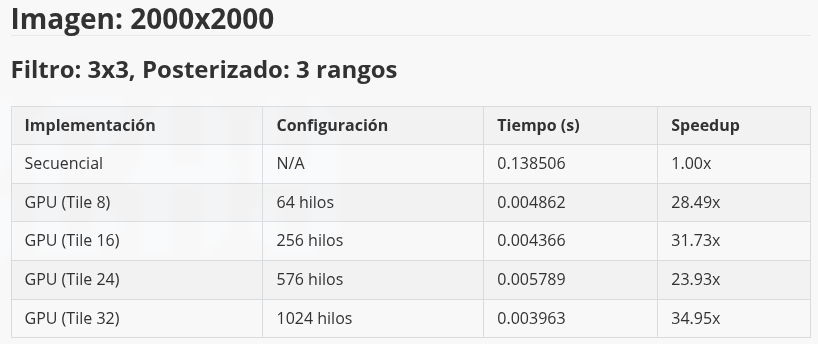
\includegraphics[width=1\textwidth]{resources/2000gpu3x3.png}
    \caption{Resultados del benchmark en entorno local para imagen de 2000x2000, filtro 3x3 y 3 rangos de posterización.}
    \label{fig:2000_local_3x3_3}
\end{figure}


\begin{figure}[H]
    \centering
    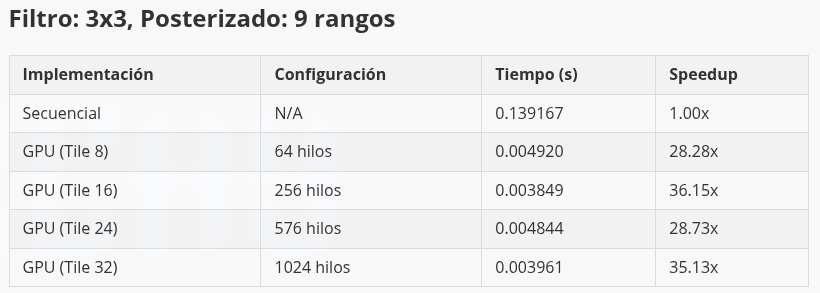
\includegraphics[width=1\textwidth]{resources/2000gpu3x9.png}
    \caption{Resultados del benchmark en entorno local para imagen de 2000x2000, filtro 3x3 y 9 rangos de posterización.}
    \label{fig:2000_local_3x3_9}
\end{figure}

\begin{figure}[H]
    \centering
    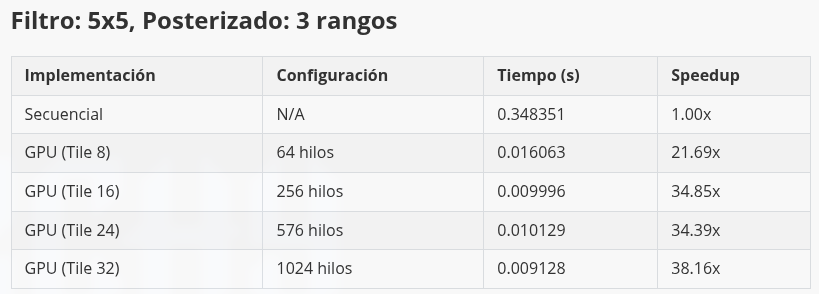
\includegraphics[width=1\textwidth]{resources/2000gpu5x3.png}
    \caption{Resultados del benchmark en entorno local para imagen de 2000x2000, filtro 5x5 y 3 rangos de posterización.}
    \label{fig:2000_local_5x5_3}
\end{figure}


\begin{figure}[H]
    \centering
    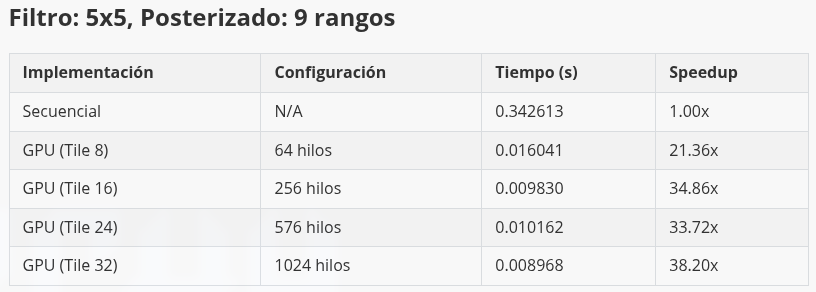
\includegraphics[width=1\textwidth]{resources/2000gpu5x9.png}
    \caption{Resultados del benchmark en entorno local para imagen de 2000x2000, filtro 5x5 y 9 rangos de posterización.}
    \label{fig:2000_local_5x5_9}
\end{figure}

% -------------------------------------------------------------------

\begin{figure}[H]
    \centering
    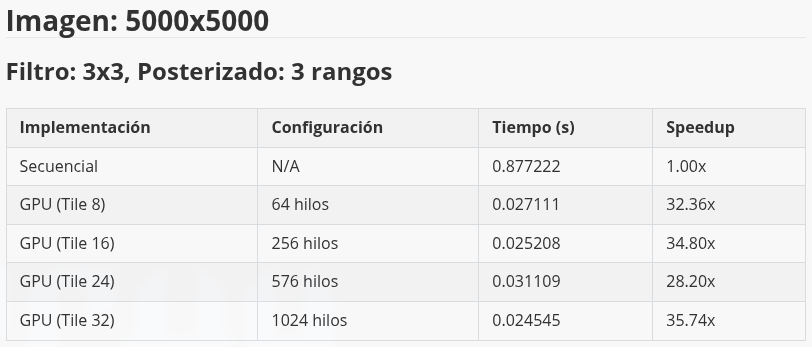
\includegraphics[width=1\textwidth]{resources/5000gpu3x3.png}
    \caption{Resultados del benchmark en entorno local para imagen de 5000x5000, filtro 3x3 y 3 rangos de posterización.}
    \label{fig:5000_local_3x3_3}
\end{figure}


\begin{figure}[H]
    \centering
    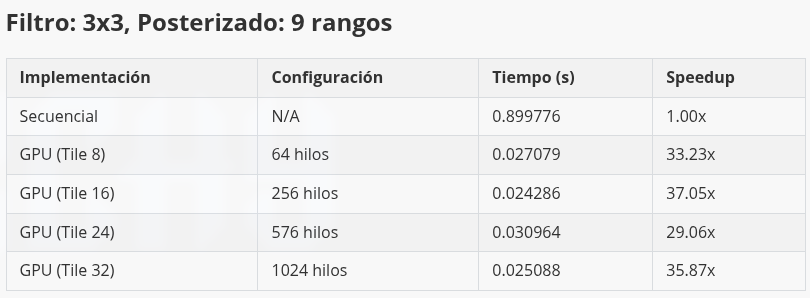
\includegraphics[width=1\textwidth]{resources/5000gpu3x9.png}
    \caption{Resultados del benchmark en entorno local para imagen de 5000x5000, filtro 3x3 y 9 rangos de posterización.}
    \label{fig:5000_local_3x3_9}
\end{figure}

\begin{figure}[H]
    \centering
    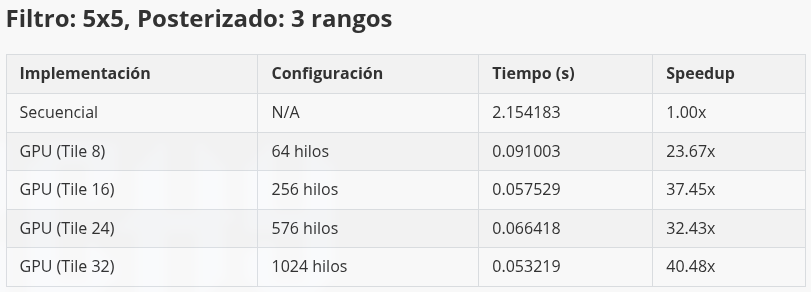
\includegraphics[width=1\textwidth]{resources/5000gpu5x3.png}
    \caption{Resultados del benchmark en entorno local para imagen de 5000x5000, filtro 5x5 y 3 rangos de posterización.}
    \label{fig:5000_local_5x5_3}
\end{figure}


\begin{figure}[H]
    \centering
    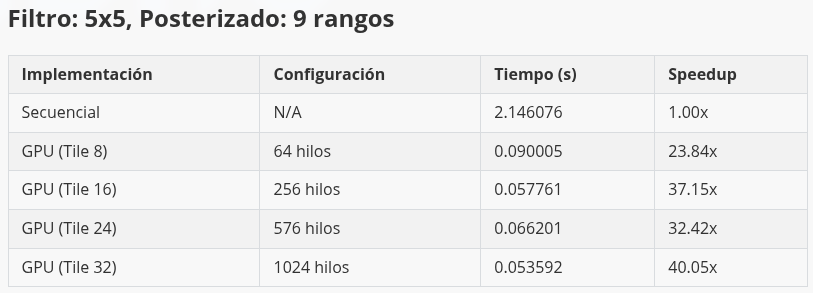
\includegraphics[width=1\textwidth]{resources/5000gpu5x9.png}
    \caption{Resultados del benchmark en entorno local para imagen de 5000x5000, filtro 5x5 y 9 rangos de posterización.}
    \label{fig:5000_local_5x5_9}
\end{figure}

